\chapter{Studi Literatur}

\section{Jaringan Komputer}
\label{sec:jaringan-komputer}

Menurut \textcite{forouzan2012}, jaringan komputer merupakan sebuah keterhubungan dari beberapa perangkat yang dapat melakukan komunikasi satu sama lain. Perangkat yang dapat terlibat pada jaringan komputer ini sapat berupa \emph{host} seperti komputer, laptop, dan gawai lainnya. Selain itu, perangkat pada definisi di atas dapat berupa perangkat penghubung. Beberapa contoh dari perangkat penghubung adalah \emph{router}, \emph{switch}, dan \emph{modem}.

Terdapat empat buah syarat sebuah sistem dapat dikatakan sebagai jaringan komputer menurut \textcite{pratama2015}. Syarat-syarat yang perlu dipenuhi adalah sebagai berikut:
\begin{enumerate}
  \item Dalam sebuah sistem, setidaknya terdapat dua buah perangkat yang terhubung. Perangkat tersebut dapat terhubung melalui sarana kabel (\emph{wired}) ataupun sarana nirkabel (\emph{wireless}).
  \item Pada sistem ini, terdapat pengguna yang melakukan interaksi dengan pengguna lainnya. Pengguna ini dapat berupa penyedia layanan atau seseorang yang hendak melakukan komunikasi melewati jaringan komputer.
  \item Pada sistem ini, terdapat data yang dipertukarkan di dalamnya. Jenis data yang dipertukarkan dapat berupa pesan teks ataupun pesan biner.
  \item Terdapat sebuah sumber daya yang digunakan secara bersama-sama. Sumber daya ini dapat berupa perangkat keras ataupun perangkat lunak.
\end{enumerate}

\subsection{Pemodelan Jaringan TCP/IP}
Menurut \textcite{odom2022}, pemodelan jaringan merupakan kumpulan dari berbagai dokumen yang menjelaskan sebuah fungsionalitas dalam sebuah jaringan. Dokumen-dokumen ini akan mendefinisikan hal-hal yang terjadi pada jaringan komputer saat bekerja. Beberapa dokumen bisa saja menjelaskan sebuah protokol jaringan, yaitu kumpulan aturan yang perlu dipenuhi saat sebuah perangkat melakukan komunikasi pada jaringan komputer.

Pemodelan jaringan TCP/IP merupakan pemodelan terbaru yang memperbaiki kekurangan yang ada pada pemodelan \emph{layer} OSI (\cite{forouzan2012}). Selain itu, munculnya pemodelan jaringan TCP/IP dikarenakan pemodelan OSI \emph{layer} sudah tidak relevan dalam pemodelan jaringan. Faktanya, Pemodelan jaringan OSI pada saat ini sudah tidak ada lagi (\cite{odom2022}), tetapi beberapa protokol pada pemodelan TCP/IP masih merujuk pada protokol asli yang ada pada \emph{layer} OSI.

Pemodelan jaringan TCP/IP dibagi menjadi lima lapisan. Menurut \textcite{forouzan2012}, lapisan tersebut di antaranya sebagai berikut:

\begin{enumerate}
  \item \emph{Application Layer}: Lapisan ini menjelaskan spesifikasi aplikasi agar dapat berkomunikasi dalam jaringan komputer. Lapisan ini berfungsi sebagai antar muka antara aplikasi dengan jaringan. Beberapa contoh protokol yang berada pada lapisan ini adalah HTTP, FTP, dan SSH.
  \item \emph{Transport Layer}: Lapisan ini menjelaskan cara untuk memecah paket data menjadi unit-unit data yang lebih kecil (yang disebut sebagai \emph{segment}). Selain itu, lapisan ini juga berfungsi untuk memberikan penomoran setiap unit paket data sehingga data yang didapatkan akan terurut saat diberikan kepada aplikasi. Beberapa contoh protokol yang bekerja pada tingkatan ini adalah TCP dan UDP.
  \item \emph{Network Layer}: Lapisan ini menjelaskan bagaimana sebuah paket data dalam melakukan proses \emph{routing} untuk mencapai tujuan. Pada lapisan ini, dikenal sebuah sistem pengalamatan yang disebut dengan IP (\emph{Internet Protocol}) yang terstandarisasi secara internasional.
  \item \emph{Data Link Layer}: Lapisan ini bertugas untuk mengkontrol data, mengontrol kesalahan pada data saat pengiriman, serta pengalamatan fisik. Pada lapisan ini juga, didefinisikan cara untuk mengontrol aliran paket (\emph{Flow Control}) pada sebuah jaringan.
  \item \emph{Physical Layer}: Lapisan ini bertugas untuk menjelaskan perangkat keras dari sebuah jaringan komputer. Selain itu, lapisna ini juga bertugas untuk membantu proses persinyalan dan sinkronisasi bit data.
\end{enumerate}

\subsection{Protokol TCP}
Menurut \textcite{pratama2015}, Protokol TCP merupakan protokol jaringan pada lapisan \emph{transport} yang bersifat dapat diandalkan (\emph{reliable}) dan berbasis koneksi (\emph{connection oriented}). TCP memiliki sifat keandalan dikarenakan adanya proses pemeriksaan \emph{segment} yang dikirimkan ke komputer tujuan. Hal ini terlihat adanya pesan berupa konfirmasi dari penerima. Selain itu, TCP merupakan protokol berbasis koneksi. Hal ini dikarenakan saat sebelum melakukan pengiriman data, protokol ini mengharuskan untuk membentuk koneksi jaringan komputer terlebih dahulu. 

Menurut \textcite{peterson2011}, Terdapat beberapa layanan yang disediakan oleh protokol TCP. Layanan-layanan tersebut memberikan jaminan pada aplikasi bahwa data yang diterima dapat dipastikan terurut dan tidak hilang. Beberapa layanan yang disediakan di antaranya adalah sebagai berikut.

% Semuanya dari peterson2011 %
\begin{enumerate}
  \item Keandalan (\emph{Reliability}): Pada protokol TCP, data yang dikirimkan terjamin keterurutan saat diterima oleh penerima. Selain itu, proses pengiriman pada TCP bersifat \emph{full-duplex}. Hal ini berarti proses pengiriman data dapat dilakukan dua arah secara bersama-sama. Pada protokol ini juga, terdapat mekanisme kontrol aliran data. Hal ini memungkinkan untuk pengirim atau penerima menentukan jumlah data yang dikirimkan dalam satu waktu.
  \item Berbasis koneksi (\emph{Connection Oriented}): Protokol TCP mengharuskan pembuatan koneksi pada saat sebelum pengiriman data. Proses pembentukan koneksi ini perlu untuk membangun koneksi tidak hanya pada pengirim dan penerima, tetapi juga pada seluruh perangkat jaringan yang terlibat. Selain itu, protokol TCP juga mengharuskan pemutusan koneksi saat komunikasi berakhir. 
  \item Layanan pengiriman alir: Pada TCP, aplikasi memungkinkan untuk mengirimkan \emph{byte-byte} data menuju aliran jaringan. TCP akan menentukan seberapa banyak data yang akan dikirimkan menuju penerima.
\end{enumerate}

Menurut \textcite{pratama2015}, terdapat tiga tahap koneksi yang perlu dilakukan saat mengirimkan data. Ketiga tahap tersebut adalah pembentukan koneksi, pengiriman data, serta terminasi koneksi. Ketiga tahap ini perlu dilakukan dikarenakan sifat dari protokol TCP yaitu berbasiskan koneksi.

Tahap pertama yang perlu dilakukan dalam mengirim data melalui TCP adalah pembentukan koneksi. Proses pembentukan koneksi dilakukan dengan menggunakan \emph{three way handshake}. Menurut \textcite{peterson2011}, \emph{server} membentuk koneksi pasif dengan \emph{client}. Selanjutnya, \emph{client} mengirimkan \emph{segment} ACK menuju server. Setelah server menerima \emph{segment} ACK, server akan mengirimkan \emph{segment} SYN+ACK. Setelah itu, \emph{client} mengirimkan \emph{segment} ACK menuju \emph{server}. Setelah semua proses ini terjadi, koneksi antar \emph{client} dan \emph{server} telah terjalin. Proses ini dapat digambarkan pada \ref{fig:tcp.open}. 

\begin{figure}[!h]
  \centering
  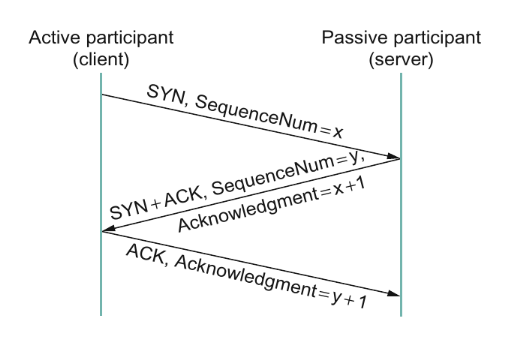
\includegraphics[width=280px]{chapters/res/chapter-2/img/tcp.open.png}
  \caption{Proses Pembukaan Koneksi TCP} \label{fig:tcp.open}
  Sumber: \textcite{peterson2011}
\end{figure}

Saat koneksi telah terjalin, pengiriman data sudah dapat dilakukan. Proses transfer data dilakukan dengan mengirimkan \emph{segment} data menuju penerima. Saat menerima data, penerima harus mengirimkan \emph{segment} ACK menuju pengirim. Apabila terjadi kegagalan transmisi, setiap \emph{segment} yang hilang harus ditransmisikan ulang.

Menurut \textcite{peterson2011}, setiap \emph{segment} yang dikirimkan diharapkan selalu penuh. Hal ini mencegah terjadi permasalahan \emph{silly window syndrome}. Oleh karena itu, pengiriman dapat diatur oleh algoritme nagle. Terdapat sebuah parameter untuk menentukan besar maksimum data yang dikirimkan yaitu nilai \emph{maximum segment size} (MSS).

Pada saat pengiriman data, terdapat juga sebuah nilai $Timeout$ yang menentukan apakah proses pengiriman \emph{segment} perlu diulang. Nilai ini dapat diturunkan melalui nilai estimasi \emph{round time trip} (RTT) dari sebuah data. Saat mengirimkan data, pengirim perlu menunggu ACK hingga batas $timeout$. Apabila telah terjadi timeout, pengirim perlu mengirimkan ulang data mereka menuju penerima. Semua proses pada tahap pengiriman ini perlu dilakukan hingga semua data berhasil dikirimkan.

Pada fase terakhir, koneksi antara \emph{client} dan \emph{server} perlu ditutup. Hal ini perlu dilakukan dengan \emph{client} melakukan proses \emph{active close}. Pada tahap \emph{active close}, \emph{client} mengirimkan pesan FIN. Setelah itu, \emph{server} mengirimkan pesan FIN+ACK. Setelah menerima pesan dari \emph{server}, \emph{client} perlu mengirimkan ACK. Setelah itu, koneksi antara \emph{server} dan \emph{client} telah tertutup.

\section{Kriptografi}
Menurut \textcite{schneier1996}, Kriptografi merupakan ilmu pengetahuan dan seni yang berujuan untuk menjaga sebuah pesan tetap aman. Menurut \textcite{anderson2008}, Kriptografi dianggap sebagai pintu para pengembang keamanan untuk bertemu dengan ilmu matematika. Hal ini dapat terlihat bahwa banyak sekali algoritme kriptografi yang terkait dengan konsep matematika. Kriptografi dianggap juga sebagai seni. Menurut \textcite{munir2019}, hal ini dikarenakan dari pandangan sejarah berkembangnya kriptografi. Kriptografi ini terbentuk dikarenakan adanya keinginan untuk merahasiakan sebuah pesan. Tentu saja, setiap orang memiliki ciri khas serta caranya tersendiri untuk menyandikan sebuah pesan. Oleh karena itu, kriptografi dapat dianggap sebagai seni untuk merahasiakan sebuah pesan. 

Kriptografi pada dasarnya memiliki beberapa layanan dasar yang dapat digunakan dalam dunia keamanan. Menurut \textcite{schneier1996}, beberapa layanan yang terdapat pada kriptografi adalah sebagai berikut:
\begin{enumerate}
  \item Kerahasiaan (\emph{confidentiality}) merupakan sebuah layanan yang diberikan oleh kriptografi untuk menjaga pesan agar pesan hanya dapat dimengerti oleh pihak yang memiliki otoritas. 
  \item Integritas (\emph{integrity}) merupakan layanan yang menjamin bahwa pesan yang diterima merupakan pesan yang belum pernah dilakukan modifikasi sebelumnya. Layanan ini menjamin data yang diterima sama dengan data tersebut saat pertama kali dikirim.
  \item Otentikasi (\emph{authentication}) merupakan layanan yang menjamin bahwa pesan yang diterima merupakan pesan yang dikirim oleh pengirim sesungguhnya. Hal ini terkait dengan klaim bahwa pesan yang dikirimkan tentu saja dapat dilakukan dekripsi dengan kunci yang telah disepakati.
  \item Anti penyangkalan (\emph{non-repudiation}) merupakan layanan yang menjamin bahwa pengirim tentu saja tidak akan dapat menyangkal pesan yang telah dia kirimkan.
\end{enumerate} 

Kriptografi modern, menurut \textcite{munir2019}, merupakan kriptografi yang bekerja pada komputer digital. Pesan tidak hanya terbatas pada tulisan dan alfabet, namun pesan juga dapat berupa berbentuk apapun selama dapat diubah menjadi bentuk biner. Dalam Kriptografi modern, terdapat sebuah konsep yang disebut dengan kriptografi kunci publik, konsep fungsi \emph{hash}, serta tanda tangan digital. Hal ini merupakan konsep baru yang dapat digunakan untuk menjamin integritas serta anti penyangkalan dari pengirim pesan.

Menurut \textcite{schneier1996}, keamanan kriptografi modern tidak hanya cukup apabila merahasiakan algoritme penguncian. Hal ini dikarenakan apabila sebuah algoritme penguncian dapat dipecahkan, algoritme tersebut perlu diganti dengan yang baru. Dalam kriptografi modern, kerahasiaan yang perlu dijaga terletak pada kunci. Setiap operasi enkripsi serta dekripsi tentu saja akan melibatkan kunci ini. 

Sebuah algoritme kriptografi tentu membutuhkan kunci untuk melakukan proses enkripsi dan dekripsi. Menurut \textcite{schneier1996}, algoritme kriptografi dapat dibagi menjadi dua, yaitu Kriptografi kunci simetrik dan kriptografi publik. Perbedaan dari kedua algoritme tersebut terletak pada kunci yang digunakan untuk melakukan enkripsi serta dekripsi pesan. 

Menurut \textcite{munir2019}, algoritme kunci simetri menggunakan kunci yang sama saat melakukan proses enkripsi serta dekripsi pesan. Asumsi yang diterapkan pada penggunaan algoritme ini adalah pengirim serta penerima sudah melakukan proses pembagian kunci. Skema proses enkripsi digambarkan pada gambar \ref{fig:crypto.symetric}.

\begin{figure}[!h]
  \centering
  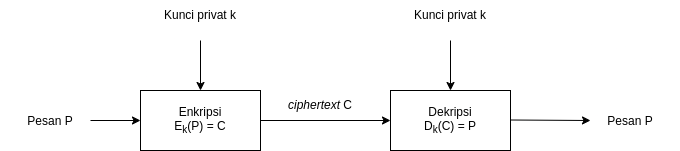
\includegraphics[width=\textwidth]{chapters/res/chapter-2/img/crypto.symetric.png}
  \caption{Visualisasi Proses Enkripsi Kriptografi Kunci Simetri} \label{fig:crypto.symetric}
  Sumber: \textcite{munir2019}
\end{figure}

Menurut \textcite{munir2019}, algoritme kriptografi kunci simetris ini dibagi lagi menjadi dua buah jenis, yaitu \emph{cipher} blok dan \emph{cipher} alir. Perbedaan antara kedua jenis \emph{cipher} tersebut terletak pada cara pengenkripsian sebuah pesan. Pada \emph{cipher} alir, proses enkripsi dilakukan dengan cara mengenkripsikan pesan per bit per bit. Proses penenkripsian juga tidak menutup kemungkinan dilakukan \emph{byte} per \emph{byte}. Contoh algoritme yang termasuk dalam \emph{cipher} alir adalah RC4 dan A5.

Menurut \textcite{munir2019}, Algoritme \emph{cipher} blok merupakan algoritme kunci simetris yang memproses pesan berdasarkan blok-blok bit atau \emph{byte}. Enkripsi dilakukan pada blok tersebut setiap kali. Terdapat beberapa operasi yang ada pada \emph{cipher} blok, di antaranya adalah ECB, CBC, CFB, dan CTR. Setiap operasi ini menentukan cara setiap blok pesan \emph{plaintext} atau \emph{ciphertext} dilakukan proses kriptografi.


\begin{figure}[!h]
  \centering
  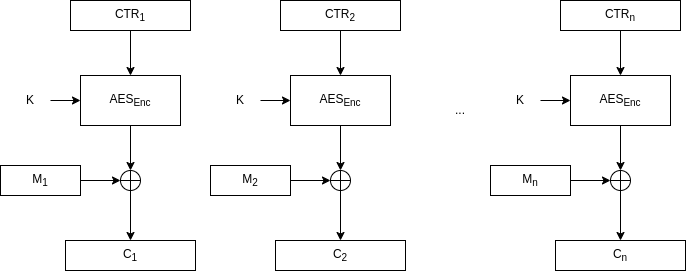
\includegraphics[width=\textwidth]{chapters/res/chapter-2/img/ctr.enc.png}
  \caption{Visualisasi Enkripsi Mode Blok CTR} 
  \label{fig:crypto.ctr.encrypt}
  Sumber: \textcite{munir2019}
\end{figure}

\begin{figure}[!h]
  \centering
  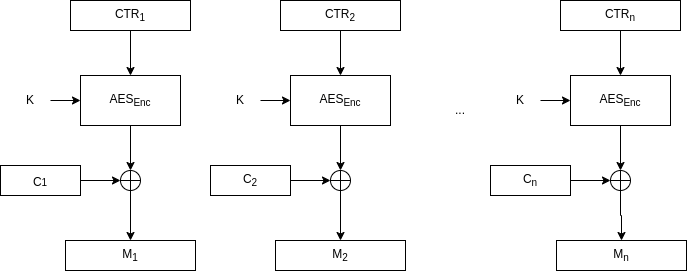
\includegraphics[width=\textwidth]{chapters/res/chapter-2/img/ctr.dec.png}
  \caption{Visualisasi Dekripsi Mode Blok CTR} 
  \label{fig:crypto.ctr.decrypt}
  Sumber: \textcite{munir2019}
\end{figure}

Salah satu bentuk mode blok yang sering digunakan dalam melakukan enkripsi adalah CTR (Counter). Menurut \textcite{munir2019}, mode enkripsi counter memanfaatkan sebuah counter yang digunakan sebagai generator dari aliran kunci. Proses enkripsi dilakukan dengan melakukan XOR antara blok pesan dengan aliran kunci. Proses ini cukup mirip dengan cipher alir. Nilai counter pada suatu blok dibangkitkan melalui proses \emph{increment} pada blok sebelumnya. Secara matematis, proses enkripsi dan dekripsi dinyatakan pada persamaan \ref{eq:crypto.ctr}.

\begin{equation}
  \label{eq:crypto.ctr}
  \begin{array}{l}
    CTR_i = f(CTR_{i-1}) \\   
    Ct_i = E_K(CTR_i) \oplus Pt_i \\
    Pt_i = E_K(CTR_i) \oplus Ct_i \\
    CTR_0 = IV
  \end{array}
\end{equation}

Menurut \textcite{munir2019}, terdapat keuntungan saat menggunakan mode blok CTR dalam melakukan enkripsi. Keuntungan utamanya adalah hasil enkripsi akan memberikan hasil cipherteks yang berbeda untuk plainteks yang sama. Hal ini disebabkan aliran kunci yang dihasilkan pada masing-masing blok berbeda. Bila dibandingkan dengan mode blok berbasis CBC, mode blok CTR bebas dari serangan \emph{padding oracle}. Hal ini dikarenakan blok yang dihasilkan pada mode CTR tidak bergantung pada input plainteks ataupun cipherteks dari blok sebelumnya. Akan tetapi, untuk menjamin keamanan yang maksimal dari mode blok ini, input counter haruslah unik. Hal ini ditujukan agar aliran kunci yang dihasilkan juga unik.

Menurut \textcite{munir2019}, algoritme kunci publik (atau bisa disebut algoritme kunci nirsimetris) merupakan algoritme enkripsi yang menggunakan kunci yang berbeda pada saat melakukan proses enkripsi dan juga proses dekripsi. Pada saat melakukan komunikasi menggunakan algoritme ini, pihak yang terlibat harus memiliki satu buah kunci, yaitu kunci publik dan kunci privat. Pengirim pesan akan menggunakan kunci publik untuk mengunci pesan. Akan tetapi, penerima menggunakan kunci privat miliknya untuk membuka pesan. Dengan menggunakan algoritme ini, hanya penerima pesan yang dapat membuka pesan. Ilustrasi terkait enkripsi memanfaatkan algoritme ini terdapat pada gambar \ref{fig:crypto.asymetric}. Beberapa contoh algoritme enkripsi kunci publik adalah RSA, \emph{Elgamal}, dan DSA.

\begin{figure}[!h]
  \centering
  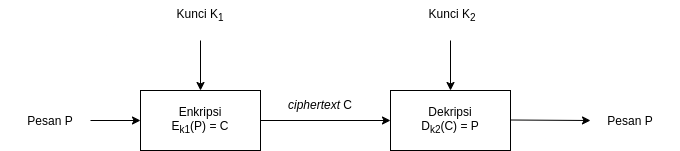
\includegraphics[width=\textwidth]{chapters/res/chapter-2/img/crypto.asymetric.png}
  \caption{Visualisasi Proses Enkripsi Kriptografi Kunci Publik} 
  \label{fig:crypto.asymetric}
  Sumber: \textcite{munir2019}
\end{figure}

Menurut \textcite{munir2019}, kriptografi kunci publik adadapat memberikan dua keuntungan. Keuntungan pertama adalah tidak adanya kebutuhan dalam mendistribusikan kunci rahasia. Kunci publik dapat dikirimkan melalui saluran yang tidak aman. Selain itu, keuntungan lain dari penggunaan kunci publik ini adalah jumlah pembuatan kunci dapat dikurangi. Pada saat menggunakan kriptografi kunci simetri, jumlah kunci yang harus dibuat adalah sebanyak jumlah pihak yang ingin berkomunikasi. Pada saat menggunakan algoritme asimetris, kunci yang perlu dibuat hanyalah sebanyak dua buah kunci, sehingga jumlah kunci menjadi lebih sedikit.

\section{Kriptografi Kurva Eliptik}
Kriptografi Kurva Eliptik pada dasarnya merupakan sebuah metode yang memanfaatkan kurva eliptik dalam melakukan proses kriptografi. Menurut \textcite{betaccini2022}, kurva eliptik adalah sebuah representasi geometri dari sebuah persamaan matematika pada bidang kartesian. Persamaan ini dinyatakan pada persamaan \ref{eq:crypto.elliptic}.

\begin{equation}
  \label{eq:crypto.elliptic}
  y^2 = x^3 + ax + b\text{ }(\text{mod} p)
\end{equation}

Menurut \textcite{munir2019}, Syarat dari persamaan ini adalah $4a^3 + 27b^2 \neq 0$. Nilai $a$ dan nilai $b$ yang berbeda dapat menghasilkan kurva eliptik yang berbeda. Keunikan dari kurva eliptik ini adalah hasil penjumlahan dari dua buah titik yang berada pada kurva eliptik akan menghasilkan titik lain yang juga berada pada kurva eliptik. Hal ini dikecualikan untuk titik $O$ yang direpresentasikan dengan titik tak hingga. Menurut \textcite{betaccini2022}, Kekuatan dari sistem krpitografi kurva eliptik terletak pada kesulitan dalam menyelesaikan persamaan diskrit logaritma. Oleh karena itu, kriptografi kurva eliptik dapat diimplementasikan pada algoritme kunci publik, seperti Diffie-Hellman.

Menurut \textcite{certicom2000}, Salah satu contoh kurva eliptik yang direkomendasikan adalah kurva eliptik secp256r1. Kurva ini didefinisikan dengan parameter pada tabel \ref{tab:crypto.secp256r1}.

\begin{table}[!h]
  \centering
  \caption{Parameter Kurva Eliptik secp256r1}
  \label{tab:crypto.secp256r1}
  \begin{tabular}{|p{1in}|p{4in}|}
    \hline
    \textbf{Parameter} & \textbf{Nilai (Dalam Heksadesimal)} \\
    \hline
    $p$ & \texttt{ffff ffff 0000 0001 0000 0000 0000 0000 0000 0000 ffff ffff ffff ffff ffff ffff} \\ \hline
    $a$ & \texttt{ffff ffff 0000 0001 0000 0000 0000 0000 0000 0000 ffff ffff ffff ffff ffff fffc} \\ \hline
    $b$ & \texttt{5ac6 35d8 aa3a 93e7 b3eb bd55 7698 86bc 651d 06b0 cc53 b0f6 3bce 3c3e 27d2 604b} \\ \hline
    $G_x$ & \texttt{6b17 d1f2 e12c 4247 f8bc e6e5 63a4 40f2 7703 7d81 2deb 33a0 f4a1 3945 d89 8c296} \\ \hline 
    $G_y$ & \texttt{4fe3 42e2 fe1a 7f9b 8ee7 eb4a 7c0f 9e16 2bce 3357 6b31 5ece cbb6 4068 37bf 51f5} \\ \hline
  \end{tabular}
\end{table}

Nilai titik $G = (G_x, G_y)$ pada tabel \ref{tab:crypto.secp256r1} merupakan titik pembangkit dari kurva eliptik secp256r1. Titik ini digunakan sebagai titik yang digunakan untuk membangkitkan titik-titik lain yang akan digunakan dalam proses kriptografi.

\section{Enkripsi Dinamis}
Enkripsi dinamis pertama kali dikenalkan oleh \textcite{knudsen2015}. Menurut \textcite{knudsen2015}, Enkripsi dinamis merupakan sebuah pendekatan kriptografi yang menyebabkan penerima pesan tidak perlu mengetahui detail proses enkripsi selain nilai dari \emph{secret key} dalam melakukan proses dekripsi. Pengirim pesan dapat menentukan algoritme enkripsi yang akan digunakan. Akan tetapi, penerima pesan tidak perlu mengetahui proses enkripsi yang dilakukan. Hal ini tentu mengharuskan bahwa penerima pesan dapat melakukan porses dekripsi dengan baik walaupun proses enkripsi tidak diketahui. 

Terdapat beberapa pendekatan yang ditawarkan oleh \textcite{knudsen2015}, salah satunya adalah dengan cara mengirimkan algoritme dekripsi $D$ ke penerima pesan. Pemilihan algoritme enkripsi dilakukan secara acak oleh pengirim. Pengiriman ini dilakukan dengan cara mengenkripsi algoritme $D$ dengan sistem enkripsi yang telah disepakati oleh kedua pihak. Penerima akan menjalankan algoritme dekripsi yang diterima untuk mendekripsi pesan. Berdasarkan \textcite{knudsen2015}, kelemahan dari pendekatan ini adalah transmisi kode \emph{executable}. Kode ini pun perlu dijalankan di penerima sehingga dapat membahayakan pengguna apabila kode yang dibuat merupakan kode yang berbahaya. Untuk mengatasi hal ini, diberikan beberapa solusi diantaranya adalah dengan memberikan pengecekan integritas dan otentikasi. Selain itu, perlu dilakukan juga pembatasan lingkungan eksekusi untuk melakukan proses dekripsi.

Menurut \textcite{knudsen2015}, terdapat varian lain dalam melakukan enkripsi dinamis, yaitu dengan menggunakan \emph{cipher} RAES. Pada \emph{cipher} RAES, proses enkripsi dilakukan sebagaimana AES-128 dilakukan. Akan tetapi, S-box yang digunakan berbeda. Terdapat dua buah kunci yang digunakan dalam melakukan enkripsi, yaitu kunci untuk digunakan pada AES-128 dan kunci untuk membangkitkan S-box. Menurut \textcite{knudsen2015}, keamanan menggunakan metode ini setidaknya sama kuatnya dengan menggunakan S-box.

\section{Pertukaran Kunci \emph{Diffie–Hellman} dengan Kurva Eliptik}
Algoritme pertukaran kunci \emph{Diffie–Hellman} dengan Kurva Eliptik merupakan algoritme yang digunakan untuk berbagi kunci sesi antara dua pihak atau lebih dengan memanfaatkan kurva eliptik. Menurut \textcite{munir2019}, algoritme pertukaran kunci ini merupakan solusi dari permasalahan kriptografi kunci simetri, yaitu pengiriman kunci pada komunikasi jaringan yang tidak aman. Secara garis besar, setiap pihak yang akan melakukan pertukaran kunci menggunakan \emph{Diffie–Hellman}, akan mengirimkan parameter publiknya kepada setiap pihak. Penerima parameter publik akan membangkitkan kunci sesi berdasarkan parameter publik yang diterima dan parameter privat yang dimiliki olehnya. Ilustrasi pertukaran kunci ini digambarkan pada gambar \ref{fig:crypto.ecdh}.

\begin{figure}[!h]
  \centering
  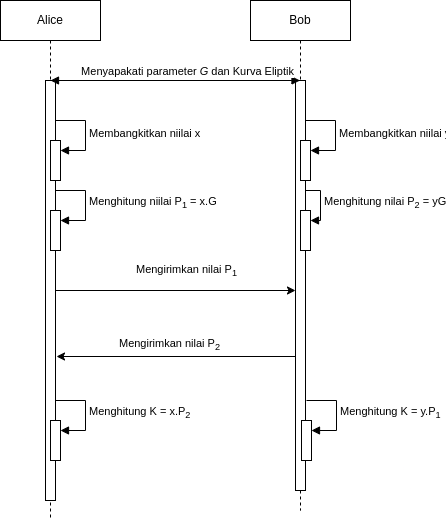
\includegraphics[width=12cm]{chapters/res/chapter-2/img/crypto.ecdh.png}
  \caption{Visualisasi Pertukaran Kunci \emph{Eliptic Curve Diffie-Hellman}} \label{fig:crypto.ecdh}
  Sumber: \textcite{munir2019}
\end{figure}

Pada ilustrasi yang ditunjukan \ref{fig:crypto.ecdh}, setiap pihak akan mendapatkan nilai $K$ yang sama. Nilai $K$ merupakan sebuah titik pada kurva eliptik yang digunakan. Nilai $K$ yang dihasilkan dari proses ini dipastikan akan sama pada kedua buah pihak. Nilai ini biasanya akan digunakan untuk membangkitkan kunci sesi yang akan digunakan pada proses enkripsi dan dekripsi pesan.

Kekuatan dari pertukaran kunci \emph{Eliptic Curve Diffie–Hellman} menurut \textcite{munir2019} terletak pada sulitnya melakukan operasi logaritma diskrit. Nilai $x$ dan $y$ yang ditunjukan pada ilustrasi \ref{fig:crypto.ecdh} hanya dapat diekstrasi bila melakukan operasi logaritma diskrit dengan basis $g$. Menurut \textcite{staling2011}, Algoritme paling baik untuk mencari nilai logaritma diskrit saat ini berada pada kompleksitas $O(e^{(\ln{p})^{1/3} \cdot (\ln{(\ln{p})})^{2/3}})$ sehingga masih belum cukup mangkus untuk menyelesaikan persoalan ini untuk nilai $p$ yang besar.

\section{\emph{Advanced Encryption Standard (AES)}}
Menurut \textcite{staling2011}, Advanced Encryption Standard (AES) merupakan sebuah salah satu algoritme cipher blok yang dibuat dengan tujuan untuk menggantikan algoritme DES. Berdasarkan panjang kunci, algoritme AES dapat dibagi menjadi tiga, yaitu AES-128, AES-192, dan AES-256. Cipher AES akan melakukan enkripsi dan dekripsi dalam sejumlah \emph{round}. Jumlah \emph{round} yang akan dilakukan bergantung terhadap panjang kunci yang digunakan. Tabel \ref{tab:aes-round} menunjukan jumlah round yang digunakan pada spesifikasi algoritme AES.

\begin{longtable}{|c|c|}
  \caption{\label{tab:aes-round} Tabel Panjang Kunci dan Jumlah Round pada Algoritme AES} \\
  \hline
  Panjang Kunci & Jumlah Round \\ \hline
  128 bit       & 10           \\ \hline
  192 bit       & 12           \\ \hline
  256 bit       & 32           \\ \hline
\end{longtable}

Menurut \textcite{staling2011}, AES memiliki empat tahap yang digunakan dalam melakukan proses enkripsi. Tahap-tahap yang dilakukan dalam algoritme \emph{Rijndael} diantaranya adalah sebagai berikut:

\begin{enumerate}
  \item Tahap \emph{AddRoundKey}\\Menurut \textcite{munir2019}, Nilai \emph{state} akan dilakukan operasi XOR terhadap \emph{round key} pada tahap ini. Nilai \emph{round key} akan dibangkitkan melalui aloritma ekspansi kunci sehingga setiap \emph{round} akan memiliki kunci yang berbeda-beda.  
  \item Tahap Transformasi \emph{ShiftRow}\\Menurut \textcite{munir2019}, Nilai \emph{state} akan dilakukan pergeseran baris matriks secara \emph{wrapping}. Operasi ini bertujuan untuk mengubah urutan dalam plainteks. Jumlah pergeseran yang dilakukan ditentukan dengan posisi elemen baris pada matriks \emph{state}.
  \item Tahap \emph{MixColumns}\\Menurut \textcite{munir2019}, tahap ini merupakan pengacakan yang dilakukan pada nilai \emph{state}. Pada tahap ini, nilai \emph{state} akan dikalikan dengan matriks tertentu. Operasi perkalian yang digunakan merupakan perkalian pada $GF(2^8)$, sedangkan operasi penjumlahan yang digunakan merupakan XOR.
  \item Tahap \emph{Subtitute Bytes}\\Menurut \textcite{munir2019}, tahap ini merupakan tahap substitusi berdasarkan sebuah tabel yang bernama S-Box. Pada tahap ini, nilai pada \emph{state} akan dipetakan nilainya berdasarkan S-box yang digunakan. AES hanya memiliki sebuah table S-box yang digunakan pada setiap putaran serta pembangkitan kunci.
\end{enumerate}

Secara garis besar, proses enkripsi melalui algoritme \emph{Rijndael} ini ditunjukan pada gambar \ref{fig:crypto.aes}.


\begin{figure}[!h]
  \centering
  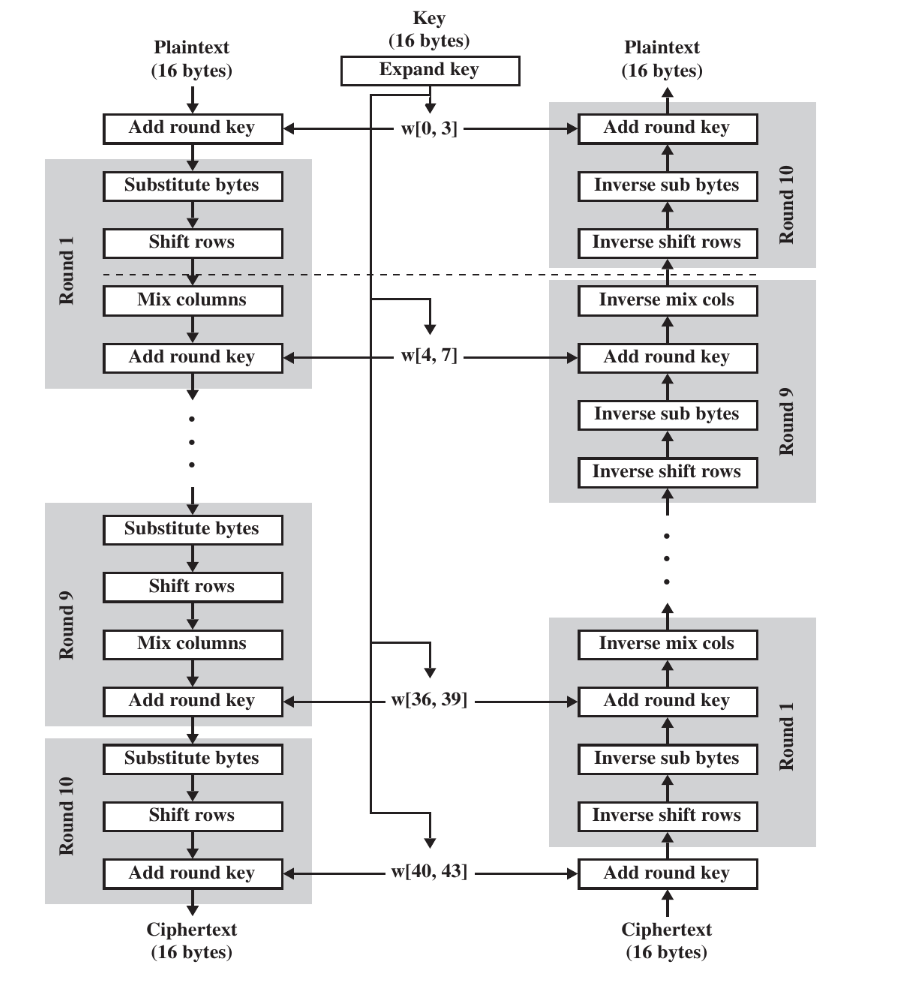
\includegraphics[width=\textwidth]{chapters/res/chapter-2/img/crypto.aes.png}
  \caption{Visualisasi Proses Enkripsi dan Dekripsi pada AES} \label{fig:crypto.aes}
  Sumber: \textcite{staling2011}
\end{figure}

\section{CSRPNG Berbasis \emph{Chaos}}
Menurut \textcite{munir2019}, Sistem chaos merupakan sistem matemtis yang dapat menghasilkan nilai dengan tidak teratur. Sistem chaos sangat peka terhadap perubahan kecil. Hal ini dikarenakan sistem chaos memiliki fenomena efek kupu-kupu.

Berdasarkan \textcite{boris2003}, terdapat tiga buah syarat sebuah sistem matematis dapat sebagai sistem chaos. Syarat tersebut diantaranya adalah sebagai berikut:
\begin{enumerate}
  \item Sistem tersebut haruslah sensitif terhadap nilai awal.
  \item Sistem tersebut harus memenuhi sifat \emph{topological transitive}. Hal ini berarti setiap nilai pada sistem chaos haruslah dapat dicapai dengan melakukan operasi sebuah fungsi secara berulang (\textcite{boris2003}).
  \item Sistem tersebut juga haruslah memiliki orbit periode yang padat.
\end{enumerate}

Menurut \textcite{munir2019}, Salah satu sifat yang dimiliki oleh sistem \emph{chaos} adalah ia bersifat deterministik. Selain itu, sistem chaos memiliki ketidakteraturan yang tinggi dalam menghasilkan nilai. SIfat yang paling penting adalah peka terhadap nilai awal. Semua sifat ini dapat memberikan sifat difusi pada algoritme kriptografi dikarenakan sistem chaos ini dapat menghilangkan hubungan statistik pada ciperteks.

Terdapat berbagai contoh dari sistem \emph{chaos} yang telah didefinisikan pada berbagai sumber. Menurut \textcite{patel2021}, Salah satu contoh fungsi \emph{chaos} yang sederhana adalah sistem \emph{chaos} berbasiskan fungsi sinus. Sistem chaos berbasis fungsi sinus didefinisikan pada persamaan \ref{eq:chaos.sin}.

\begin{equation}
  \label{eq:chaos.sin}
  X_{n+1} = \mu \cdot \sin(\pi \cdot X_n) / 4
\end{equation}

Menurut \textcite{patel2021}, Nilai awal dari sistem ini harus berada pada range $(0, 1)$. Nilai $\mu$ yang berada pada range $(3.57, 4)$ akan menghasilkan sifat \emph{chaos} pada sistem ini. Hasil bifurcation diagram pada sistem peta sinus dapat dilihat pada gambar \ref{fig:chaos.sin.bifurcation}.

\begin{figure}[!h]
  \centering
  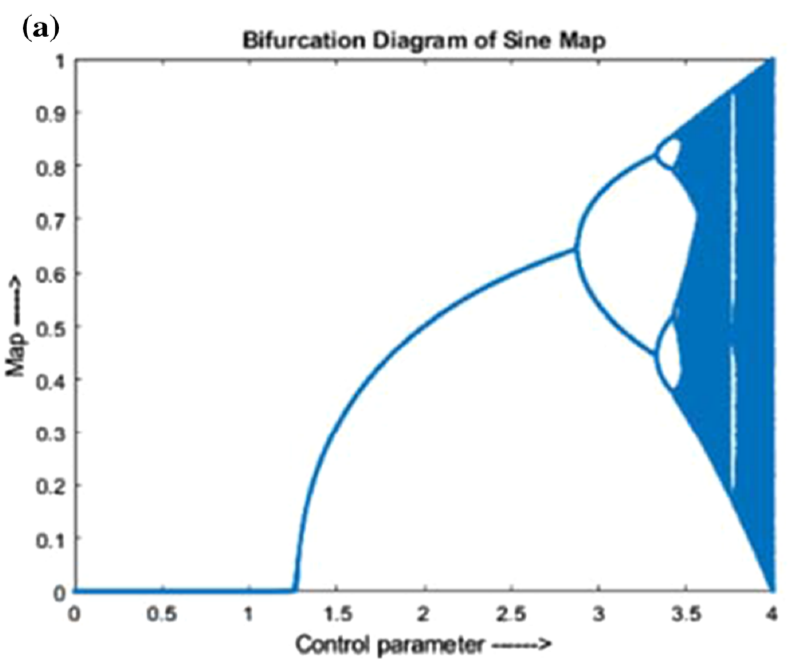
\includegraphics[width=10cm]{chapters/res/chapter-2/img/sine.bifurcation.png}
  \caption{Diagram \emph{bifurcation} pada peta sinus dengan nilai $0 \ge \mu \ge 4$} \label{fig:chaos.sin.bifurcation}
  Sumber: \textcite{patel2021}
\end{figure}


Selain sistem \emph{chaos} berbasiskan persamaan sinus, terdapat sistem chaos memanfaatkan peta hénon. Berdasarkan \textcite{henon1976}, persamaan peta hénon didefinisikan sebagaimana persamaan \ref{eq:chaos.henon}.

\begin{equation}
  \label{eq:chaos.henon}
  \begin{array}{l}   
  X_{n+1} = Y_{n} + 1 - aX_{n}^2 \\
  Y_{n+1} = bX_{n} 
  \end{array}
\end{equation}

Menurut \textcite{aybar2013}, untuk nilai $b = 0.3$ dihasilkan peta \emph{bifurcation} yang ditunjukan pada gambar \ref{fig:henon.bifurcation}. gambar \ref{fig:henon.bifurcation} memperlihatkan bahwa saat nilai $a$ mendekati $1.2$, sifat \emph{chaos} terjadi. Hal ini terjadi dikarenakan proses \emph{bifurcation} terjadi sangat cepat sehingga muncul sifat \emph{chaos} pada sistem tersebut.

\begin{figure}[!h]
  \centering
  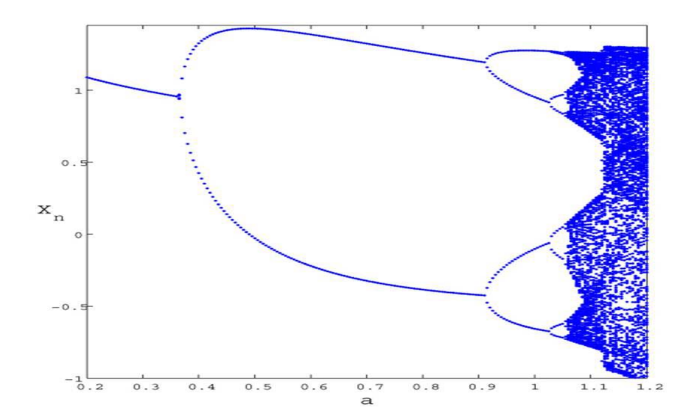
\includegraphics[width=\textwidth]{chapters/res/chapter-2/img/henon.bifurcation.png}
  \caption{Diagram \emph{bifurcation} pada peta hénon dengan nilai $0.2 \ge a \ge 1.2$ dan $b = 0.3$} \label{fig:henon.bifurcation}
  Sumber: \textcite{aybar2013}
\end{figure}

Menurut \textcite{patel2021}, terdapat metode untuk menggabungkan dua buah peta chaos. Hal ini didefinisikan pada persamaan \ref{eq:chaos.combine}.
\begin{equation}
  \label{eq:chaos.combine}
  X_{n+1} = \text{mod}(\text{A}(X_n) + \text{B}(X_n), 1)
\end{equation}

Dalam hal ini, fungsi $\text{A}$ dan $\text{B}$ merupakan dua buah fungsi chaos yang berbeda. Nilai $X_n$ merupakan nilai chaos yang dihasilkan dari sistem \emph{chaos} tersebut.
  
Menurut \textcite{munir2019}, untuk membangkitkan nilai bilangan bulat, sistem \emph{chaos} haruslah dilakukan konversi menuju bilangan bulat. Salah satu fungsi yang dapat digunakan dalam melakukan konversi ini dinyatakan pada persamaan \ref{eq:chaos.linearization}.

\begin{equation}
  \label{eq:chaos.linearization}
  T(x, n) = \lfloor x \cdot 10^n \rfloor
\end{equation}

\section{Message Authentication Code (MAC)}
Menurut \textcite{munir2019}, Fungsi hash satu arah merupakan fungsi yang dapat menghasilkan sebuah \emph{message digest} yang tidak dapat dikembalikan menjadi pesan sesungguhnya. Dua pesan berbeda dapat menghasilkan nilai hash yang berbeda. Beberapa contoh fungsi hash adalah MD5 dan SHA-256.

Menurut \textcite{munir2019}, MAC merupakan perbaikan dari permasalahan yang muncul apabila menggunakan pengecekan integritas data memanfaatkan nilai hash. Dalam menjaga integritas sebuah data dengan menggunakan nilai hash saja, dapat menimbulkan kerentanan apabila data dan nilai hash diubah. MAC merupakan sebuah fungsi \emph{hash} satu arah yang menggunakan kunci rahasia dalam pembangkitannya.

\begin{figure}[!h]
  \centering
  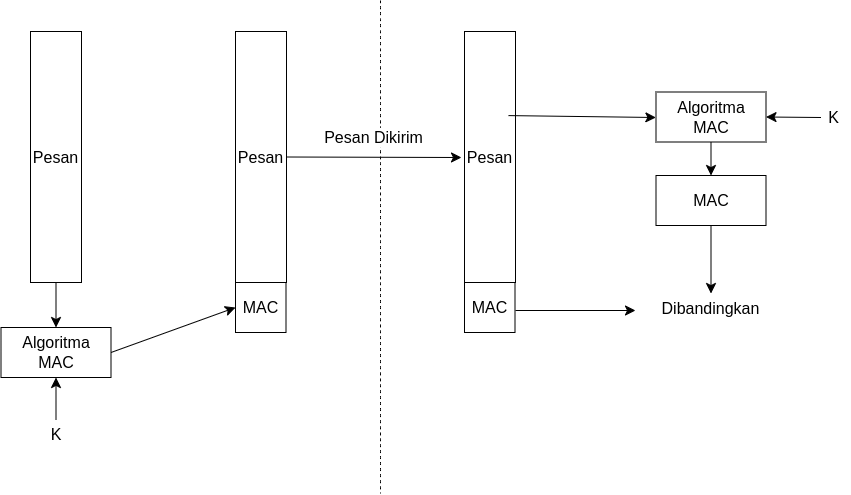
\includegraphics[width=350px]{chapters/res/chapter-2/img/mac.png}
  \caption{Ilustrasi proses pengiriman dan verifikasi pesan dengan MAC} \label{fig:mac}
  Sumber: \textcite{munir2019}
\end{figure}

Menurut \textcite{munir2019}, MAC dapat digunakan sebagai otentikasi pesan tanpa perlu melakukan enkripsi pada pesan tersebut. Hal ini dapat dilakukan dengan cara melekatkan nilai MAC pada pesan yang dikirimkan. Proses tersebut digambarkan pada gambar \ref{fig:mac}. Proses verifikasi pesan dilakukan dengan membandingkan nilai MAC dari pesan yang dihitung ulang berdasarkan pesan yang diterima dengan nilai MAC yang dikirimkan. Apabila pesan tidak diubah, kedua nilai ini menghasilkan nilai yang sama. Keuntungan menggunakan MAC ini adalah adanya nilai $K$ sehingga nilai hash yang dilekatkan pada pesan tidak secara mudah dapat diganti.

\section{Tanda Tangan Digital berbasis Kurva Eliptik}
Menurut \textcite{munir2019}, tanda tangan digital merupakan sebuah metode kriptografi yang dapat mengotentikasi pengirim dari pesan yang diterima. Dalam tanda tangan digital, terdapat beberapa layanan kriptografi yang digunakan diantaranya adalah penjagaan integritas dari data, otentikasi pengirim, serta anti penyangkalan. Tanda tangan digital ini dapat dibuat dengan dua buah cara, yaitu dengan melakukan enkripsi terhadap pesan tersebut ataupun melakukan enkripsi dari hash pesan tersebut. 

Proses tanda tangan digital pada umumnya melibatkan kriptografi kunci publik. Salah satu skema yang digunakan dalam membangkitkan tanda tangan adalah ECDSA (\emph{Eliptic Curve Digital Signature Algorithm}). Menurut \textcite{munir2019}, ECDSA merupakan sebuah skema yang diturunkan dari algoritme tanda tangan digital Elgamal. Untuk menjelaskan proses kriptografi yang dilakukan, diasumsikan terdapat dua buah entitas, yaitu Ahmad dan Budi yang akan melakukan pertukaran pesan. Ahmad akan mengirimkan pesan kepada Budi dengan dibubuhi tanda tangan digital.

Pada mulanya, Ahmad dan budi akan menyepakati kurva eliptik yang akan digunakan serta titik generator ($G$). Keduanya akan membangkitkan dua buah kunci, yaitu kunci publik dan kunci privat. Persamaan \ref{eq:ecdsa.key}, menjelaskan proses pembangkitan kunci publik dan kunci privat.

\begin{equation}
  \label{eq:ecdsa.key}
  \begin{array}{l}   
    P = x \cdot G \\
  \end{array}
\end{equation}

Kunci $P$ pada masing-masing partisipan akan saling dipetukarkan, sedangkan nilai $x$ merupakan kunci privat yang dibangkitkan secara acak. Misalkan kunci publikdari Ahmad dan Budi secara berturut-turut didefinisikan dengan $P_{A}$ dan $P_{B}$, sedangkan kunci privat mereka didefinisikan dengan $a$ dan $b$.

Saat Ahmad akan membuat tanda tangan, Ahmad perlu memilih nilai acak $k$. Nilai ini harus diambil dari rentang $[1, p-1]$. Selanjutnya, ahmad perlu menghitung nilai $r$ sesuai dengan persamaan \ref{eq:ecdsa.r}. Apabila nilai $r$ adalah 0, Ahmad perlu memilih nilai $k$ yang lain.

\begin{equation}
  \label{eq:ecdsa.key}
  \begin{array}{l}   
    Q = k \cdot G \\
    Q = (Q_x, Q_y) \\
    r = Q_x \mod p
  \end{array}
\end{equation}

Selanjutnya, Ahmad akan menghitung nilai hash dari pesan. Hasil hash pesan tersebut dinyatakan sebagai $e = H(m)$. Setelah mendapatkan nilai ini, Ahmad perlu menghitung nilai $s$ sesuai dengan persamaan \ref{eq:ecdsa.s}.

\begin{equation}
  \label{eq:ecdsa.s}
  \begin{array}{l}   
    s = k^{-1} \cdot (e + a \cdot r) \mod p
  \end{array}
\end{equation}

Nilai $(r,s)$ dikirimkan kepada budi bersamaan dengan pesan yang akan dikirimkan. Budi memverifikasi terlebih dahulu bahwa nilai $r$ dan $s$ harus berada pada selang $[1, p-1]$. Selanjutnya, Budi mengambil kunci publik Ahmad $P_{A}$. Budi akan menghitung nilai $e$ dengan cara yang sama dengan yang dilakukan oleh Ahmad. Budi juga akan menghitung nilai $w$ sesuai dengan persamaan \ref{eq:ecdsa.w}.

\begin{equation}
  \label{eq:ecdsa.w}
  \begin{array}{l}   
    w = s^{-1} \mod p
  \end{array}
\end{equation}

Dari nilai $w$, Budi perlu menghitung nilai $u_1$ dan $u_2$ sesuai dengan persamaan \ref{eq:ecdsa.u}.

\begin{equation}
  \label{eq:ecdsa.u}
  \begin{array}{l}   
    u_1 = e \cdot w \mod p \\
    u_2 = r \cdot w \mod p
  \end{array}
\end{equation}

Setelah mendapatkan nilai $u_1$ dan $u_2$, Budi perlu menghitung nilai $v$ dengan persamaan \ref{eq:ecdsa.v}.

\begin{equation}
  \label{eq:ecdsa.v}
  \begin{array}{l}   
    Q = u_1 \cdot G + u_2 \cdot P_{A} \\
    v = Q_x \mod p
  \end{array}
\end{equation}

Apabila nilai $v$ sama dengan nilai $r$, maka tanda tangan yang diberikan oleh Ahmad adalah benar. Oleh karena itu, budi dapat memastikan pesan tersebut berasal dari Ahmad.

\section{\emph{Transport Layer Security} (TLS)}
\label{sec:tls}

Menurut \textcite{rfc5246}, Protokol TLS merupakan protokol yang dapat memberikan perlindungan data baik secara privasi dan juga terhadap integritas dari sebuah data. Pada dasarnya protokol ini merupakan pengembangan dari protokol SSL. Protokol TLS terdiri atas dua buah layer, yaitu protokol \emph{Handshake} dan protokol \emph{Record}. Secara singkat, layer \emph{Handshake} menjelaskan terkait cara untuk menyamakan \emph{state} dari setiap partisipan. Pada layer \emph{Record}, dijelaskan terkait cara untuk membungkus pesan yang akan dikirimkan. Protokol TLS harus bekerja diatas layer transport yang reliabel. Transport yang digunakan biasanya adalah TCP.

Menurut \textcite{munir2019}, Protokol TLS ini merupakan pengembangan dari protokol SSL yang dikembangkan oleh Netscape pada tahun 1994. Protokol ini dikembangkan untuk mengatasi kelemahan yang dimiliki oleh SSL. Protokol ini memiliki beberapa versi, diantaranya adalah TLS 1.0, TLS 1.1, TLS 1.2, dan TLS 1.3. 

Protokol TLS 1.2 merupakan protokol yang paling banyak digunakan pada saat ini. Protokol ini memiliki beberapa fitur yang tidak dimiliki oleh protokol SSL dan TLS sebelumnya:
\begin{enumerate}
  \item Protokol TLS 1.2 mendukung HMAC berbasis SHA256
  \item Protokol TLS 1.2 tidak lagi mendukung \emph{cipher} yang tidak aman, seperti DES dan IDEA.
  \item PRF berbasiskan MD4/SHA-1 digantikan dengan PRF berbasis P\_SHA256.
  \item Adanya \emph{cipher} baru seperti AES-GCM.
\end{enumerate}

Protokol TLS 1.3 merupakan protokol yang paling baru dari protokol TLS. Berdasarkan \textcite{rfc8446}, Protokol ini menawarkan optimasi proses handshake dari TLS 1.2. Selain itu, protokol ini juga hanya mendukung \emph{cipher} berbasis \emph{Authenticated Encryption with Associated Data} (AEAD).


\subsection{Protokol \emph{Handshake}}
\label{sec:tls.handshake}

Proses \emph{Handshake} merupakan proses untuk menyamakan \emph{state} dari kedua partisipan yang terkoneksi melalui protokol TLS. Proses ini dilakuan setelah koneksi TCP berhasil dibuat. Secara umum, proses handshake
digambarkan pada gambar \ref{fig:tls.handshake}.

\begin{figure}[!h]
  \centering
  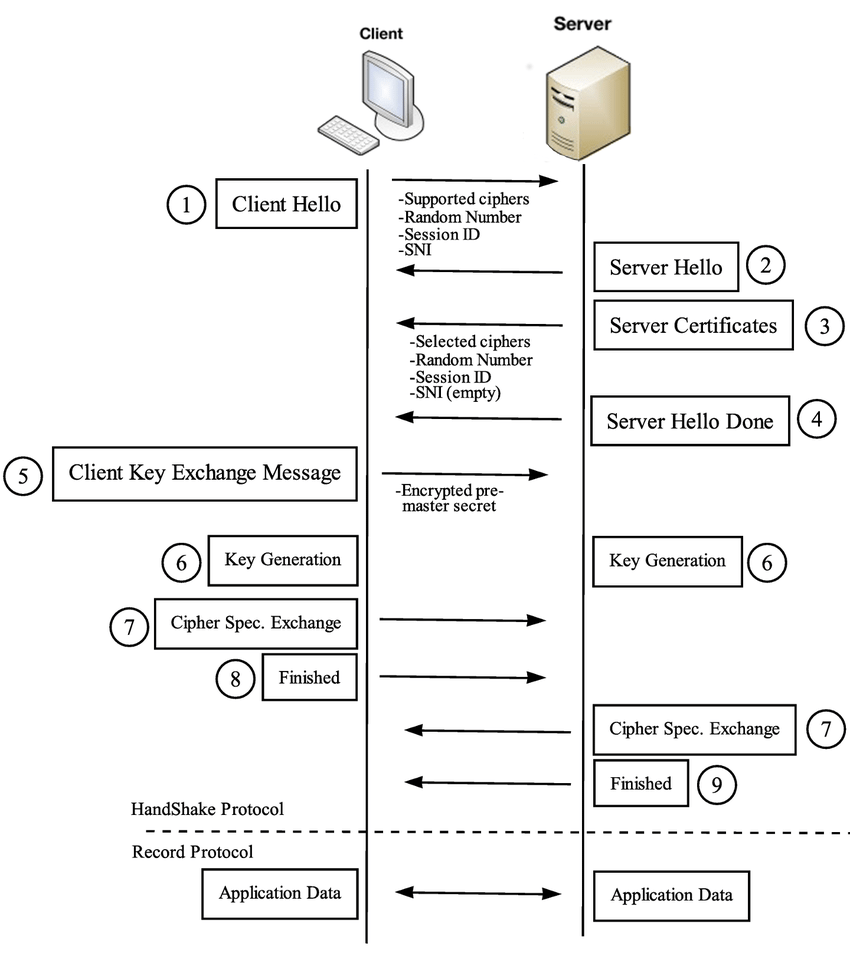
\includegraphics[width=350px]{chapters/res/chapter-2/img/tls.protocol.png}
  \caption{Ilustrasi protokol TLS} \label{fig:tls.handshake}
  Sumber: \textcite{shbair2016}
\end{figure}

\subsubsection{Pesan \emph{Hello} dan Sertifikat Digital}
Menurut \textcite{rfc5246}, proses handshake diawali dengan mengirimkan pesan berupa \emph{client hello}. Pesan ini diilustrasikan pada gambar \ref{fig:tls.clienthello}. Pesan ini setidaknya berisi beberapa nilai sebagai berikut:
\begin{enumerate}
  \item Versi dari protokol TLS yang digunakan.
  \item Waktu \emph{client} saat ini.
  \item Nilai random $r_c$ yang dibangkitkan oleh \emph{client}.
  \item Daftar cipher yang didukung oleh \emph{client}.
  \item Daftar kompresi yang didukung oleh \emph{client}.
  \item Daftar ekstensi yang dipesan oleh \emph{client}.
\end{enumerate}

\begin{figure}[!h]
  \centering
  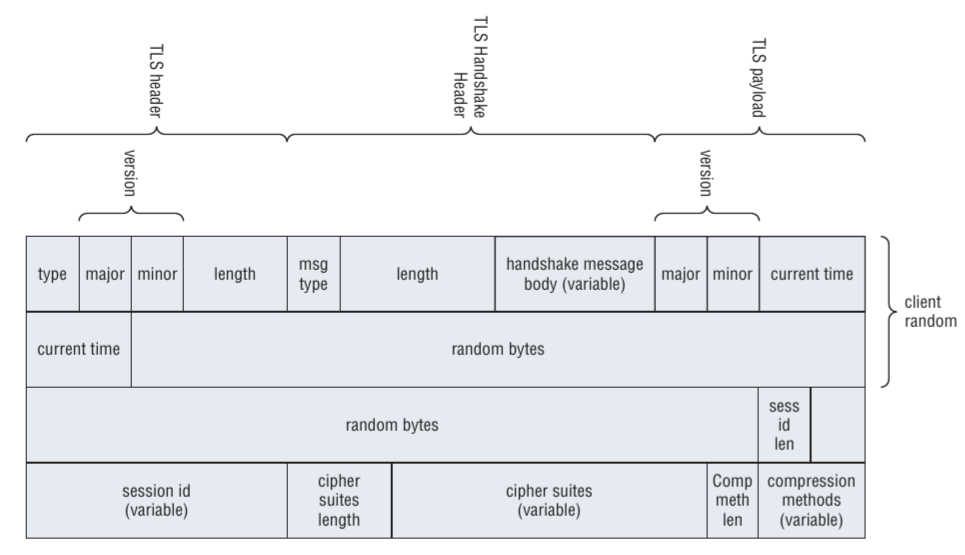
\includegraphics[width=350px]{chapters/res/chapter-2/img/tls.hello.client.png}
  \caption{Ilustrasi pesan \emph{client hello}} \label{fig:tls.clienthello}
  Sumber: \textcite{joshua2011}
\end{figure}

\begin{figure}[!h]
  \centering
  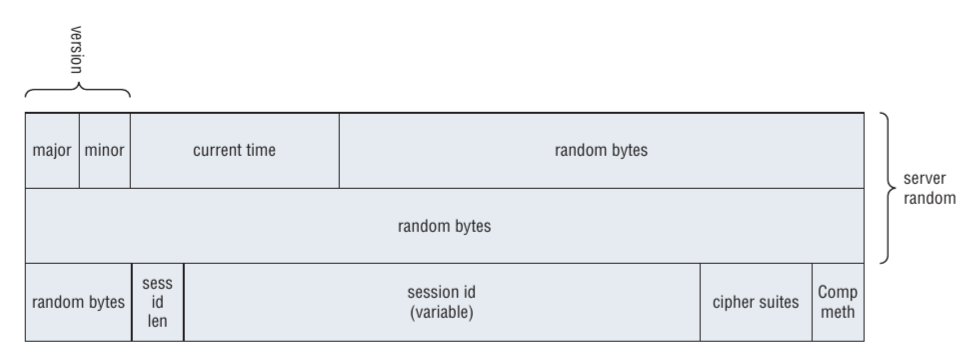
\includegraphics[width=350px]{chapters/res/chapter-2/img/tls.hello.server.png}
  \caption{Ilustrasi pesan \emph{server hello}} \label{fig:tls.serverhello}
  Sumber: \textcite{joshua2011}
\end{figure}

 Daftar cipher standard didefinisikan pada \textcite{rfc5246}. Menurut \textcite{rfc5246}, cipher suite yang diawali oleh bit $0xff$ merupakan cipher suite yang dapat digunakan untuk lingkungan privat. Selain itu, dijelaskan juga beberapa cipher lain yang memanfaatkan Eliptic Curve pada \textcite{rfc4492}. 

Setelah menerima pesan \emph{client hello}, \emph{server} akan mengirimkan pesan \emph{server hello}. Pesan ini diilustrasikan pada gambar \ref{fig:tls.serverhello}. Pesan ini setidaknya berisi beberapa nilai sebagai berikut:
\begin{enumerate}
  \item Versi dari protokol TLS yang digunakan.
  \item Waktu \emph{server} saat ini.
  \item Nilai random $r_s$ yang dibangkitkan oleh server 
  \item Cipher suite yang dipilih oleh server dari daftar cipher yang didukung oleh \emph{client}.
  \item Metode kompresi yang dipilih oleh server dari daftar kompresi yang didukung oleh \emph{client}.
  \item Ekstensi yang akan digunakan oleh \emph{server}.
\end{enumerate}

Nilai random $r_c$ dan $r_s$ akan digunakan saat membangkitkan \emph{premaster secret} yang akan diturunkan sebagai kunci enkripsi dan dekripsi.

Pesan pendukung lain yang perlu dikirimkan oleh \emph{server} adalah sertifikat digital \emph{server} yang digunakan oleh \emph{server}. Sertifikat ini akan dilakukan proses encoding dengan format DER pada sertifikat dengan format X509v3. Sertifikat yang dikirimkan dapat lebih dari satu untuk menyatakan \emph{chain of trust} dari sertifikat tersebut. Fungsi dari sertifikat digital ini adalah sebagai media otentikasi dari server tersebut.


\subsubsection{Pertukaran Kunci}
\label{sec:tls.keyexchange}

Pada dasarnya, TLS mendukung dua metode pertukaran kunci sebagai berikut:
\begin{enumerate}
  \item RSA\\
  Pada mulanya, client akan membangkitkan \emph{premaster secret}. Nilai ini kemudian akan dikirimkan ke server dengan melakukan enkripsi memanfaatkan kunci publik dari sertifikat digital yang telah diterima oleh client. Server akan mendekripsi nilai ini dengan menggunakan kunci privat yang dimilikinya.

  \item Diffie-Hellman\\
  Pada metode ini, server akan mengirimkan parameter Diffie-Hellman kepada \emph{client}. Selanjutnya, \emph{client} akan mengirimkan juga parameter Diffie-Hellman yang digunakan. Setelah itu, kedua pihak akan membangkitkan nilai \emph{premaster secret} berdasarkan hasil pada proses Diffie-Hellman. Metode pertukaran ini dapat diperluas menggunakan kurva eliptik sebagaimana yang dijelaskan pada RFC 4492. 
\end{enumerate}

Menurut \textcite{rfc5246} saat menggunakan pertukaran kunci Diffie-Hellman, pesan dari \emph{server} harus ditambahkan tanda tangan digital. Hal ini menjamin bahwa parameter Diffie-Hellman yang digunakan adalah benar-benar berasal dari \emph{server} sesungguhnya. 

\subsubsection{Pembangkitan Kunci}
Dalam membangkitkan \emph{master key}, diperlukan sebuah fungsi $\text{PRF}$ yang didefinisikan pada persamaan \ref{eq:tls.prf}.

\begin{equation}
  \label{eq:tls.prf}
  \begin{array}{l}   
    \text{PRF}(K, L, S) = \text{P}_\text{hash}(K, L || S)
  \end{array}
\end{equation}

Pada persamaan \ref{eq:tls.prf}, nilai $K$ merupakan nilai kunci dari PRF yang digunakan. Nilai $L$ merupakan label yang digunakan dalam membangkitkan nilai. Nilai $S$ adalah nilai seed yang digunakan dalam membangkitkan PRF. Operator $||$ merupakan operator untuk melakukan \emph{concatenation}. Fungsi $\text{P}_\text{Hash}$ merupakan fungsi yang didefinisikan pada persamaan \ref{eq:tls.ph}.

\begin{equation}
  \label{eq:tls.ph}
  \begin{array}{l}   
    \text{P}_\text{Hash}(K, S) = \text{HMAC}_\text{Hash}(K, A(1, S)\text{ }||\text{ }S)\text{ }||\text{ }
        \text{HMAC}_\text{Hash}(K, A(2, S)\text{ }||\text{ }S)\text{ }||\text{ }\ldots
  \end{array}
\end{equation}

Pada persamaan \ref{eq:tls.ph}, nilai $A$ adalah nilai keadaan yang didefinisikan pada persamaan \ref{eq:tls.a}. Hash yang digunakan pada proses ini adalah hash yang digunakan pada cipher suite yang dipilih. Pada umumnya, hash yang digunakan adalah SHA-256. Jumlah pengulangan pada fungsi $P$ dilakukan hingga bit-bit yang dihasilkan telah mencukupi.

\begin{equation}
  \label{eq:tls.a}
  \begin{array}{l}   
    A(i, S) = \text{HMAC}_\text{Hash}(K, A(i-1, S)\text{ }||\text{ }S) \\
    A(0, S) = S
  \end{array}
\end{equation}

Setelah mendapatkan nilai \emph{premaster secret} ($PM$), kedua partisipan perlu membangkitkan \emph{master secret}. Persamaan \ref{eq:tls.master} menjelaskan proses pembangkitan \emph{master secret} ($M$) yang diturunkan dari \emph{premaster secret}.

\begin{equation}
  \label{eq:tls.master}
  \begin{array}{l}
    M = \text{PRF}(PM, \text{"master secret"}, r_c \text{ }||\text{ }r_s)[0:47]
  \end{array}
\end{equation}

Menurut \textcite{rfc5246}, Hasil dari fungsi PRF pada perhitungan diatas perlu dilakukan pemotongan hingga indeks 47. Kegunaan dari nilai \emph{master key} adalah untuk membangkitkan kunci enkripsi. Nilai \emph{master secret} ini akan digunakan sebagai pembangkit parameter-parameter berikut:

\begin{enumerate}
  \item \emph{Client write mac key} yang digunakan oleh client untuk sebagai kunci MAC pada pesan yang dikirimkan.
  \item \emph{Server write mac key} yang digunakan oleh server untuk sebagai kunci MAC pada pesan yang dikirimkan.
  \item \emph{Client write key} yang digunakan oleh client sebagai kunci enkripsi pesan yang dikirimkan.
  \item \emph{Server write key} yang digunakan oleh server sebagai kunci enkripsi pesan yang dikirimkan.
  \item \emph{Client write IV} yang digunakan oleh client sebagai \emph{initialization vector} pada proses enkripsi.
  \item \emph{Server write IV} yang digunakan oleh server sebagai \emph{initialization vector} pada proses enkripsi.
\end{enumerate}

Nilai-nilai tersebut dibangkitkan dengan cara mempartisi kunci blok $B$ pada persamaan \ref{eq:tls.b} menjadi beberapa bagian.

\begin{equation}
  \label{eq:tls.b}
  \begin{array}{l}
    B = \text{PRF}(M, \text{"key expansion"}, r_c \text{ }||\text{ }r_s)
  \end{array}
\end{equation}

\subsubsection{Verifikasi \emph{Handshake}}
Setelah kedua pihak berhasil membangkitkan kunci, keduanya akan mengirimkan pesan \emph{change cipher spec}. Pesan ini menandakan bahwa pihak pengirim telah membangkitkan kunci yang nantinya akan digunakan. Setelah pesan ini dikirimkan, proses pengiriman pesan sudah dapat dilakukan secara terenkripsi. 

Dalam TLSv1.2, terdapat pesan tambahan yang dikirimkan oleh \emph{client} dan \emph{server} yang berupa pesan \emph{finished}. Pesan ini haeus dikirimkan setelah pesan \emph{change cipher spec} dikirimkan. Pesan ini ditujukan untuk melakukan verifikasi bahwa proses \emph{handshake} telah berhasil dilakukan.

Pesan \emph{finished} berisi sebuah nilai $V$ yang dihasilkan dari fungsi PRF. Persamaan \ref{eq:tls.finished} menjelaskan proses pembangkitan nilai $V$.

\begin{equation}
  \label{eq:tls.finished}
  \begin{array}{l}
    V = \text{PRF}(M, L, \text{Hash}(\text{handshake message}))
  \end{array}
\end{equation}

Pada pembangkitan nilai $V$, nilai \emph{handshake message} merupakan nilai hash dari seluruh pesan bertipe \emph{handshake} yang dikirimkan ataupun diterima. Nilai ini harus berurutan berdasarkan waktu penerimaan ataupun pengiriman pesan tersebut. Panjang yang dibutuhkan untuk nilai $V$ bergantung pada \emph{cipher suite} yang digunakan. Panjang dari nilai $V$ minimal adalah 12 bytes.

Nilai $L$ bergantung terhadap peran dari partisipan. Nilai $L$ yang digunakan oleh \emph{client} adalah "client finished", sedangkan nilai $L$ yang digunakan oleh \emph{server} adalah "server finished".

\subsection{\emph{Record Layer}}
Record layer menjelaskan terkait cara sebuah pesan dapat dibungkus dalam sebuah fragment TLS. Menurut \textcite{rfc5246}, Pada layer ini dijelaskan bahwa pesan pada mulanya harus dipecah dengan panjang tiap-tiap fragment maksimal adalah $2^14$ bytes. Setiap pesan yang telah dipecah menjadi beberapa fragment akan dibungkus dengan header sehingga memiliki informasi sebagai berikut:

\begin{enumerate}
  \item \emph{Content Type} menunjukan tipe dari pesan yang dikirimkan.
  \item \emph{Protocol Version} menunjukan versi dari protokol TLS yang digunakan.
  \item \emph{Length} menunjukan panjang dari pesan yang dikirimkan dalam bytes.
  \item \emph{Data} merupakan pesan yang dikirimkan.
\end{enumerate}

Ilustrasi dari struktur data pesan ini ditunjukan pada gambar \ref{fig:tls.record}. Menurut \textcite{rfc5246}, Nilai \emph{Content Type} yang digunakan pada protokol TLS dituliskan pada tabel \ref{tab:tls.contenttype}.

\begin{table}[!h]
  \centering
  \caption{Nilai \emph{Content Type} pada protokol TLS} \label{tab:tls.contenttype}
  \begin{tabular}{|c|c|}
    \hline
    \textbf{Nilai (Desimal)} & \textbf{Nama Pesan} \\
    \hline
    20 & \emph{Change Cipher Spec} \\ \hline
    21 & \emph{Alert} \\ \hline
    22 & \emph{Handshake} \\ \hline
    23 & \emph{Application Data} \\
    \hline
  \end{tabular}
\end{table}

\begin{figure}[!h]
  \centering
  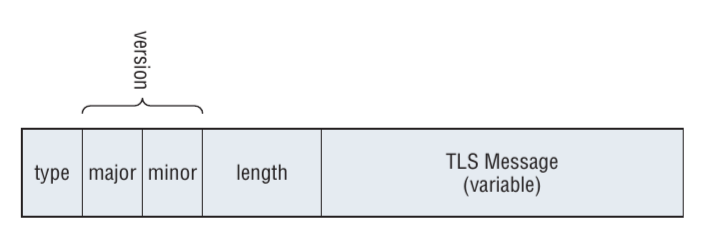
\includegraphics[width=350px]{chapters/res/chapter-2/img/tls.record.png}
  \caption{Ilustrasi struktur data pesan pada layer record} \label{fig:tls.record}
  Sumber: \textcite{joshua2011}
\end{figure}

\section{NIST Statistical Test Suite}
\label{sec:nist.statistical.test}

Menurut \textcite{rukhin2010}, NIST Statistical Test Suite merupakan kumpulan dari beberapa tes statistik yang digunakan untuk menguji kualitas keamanan dari sebuah barisan bilangan acak terhadap ancaman statistik. Sebuah sistem penghasil bilangan acak perlu memiliki sifat keteracakan dan sifat \emph{unpredictability}. 

Sifat keteracakan adalah kondisi dimana setiap bit yang dihasilkan oleh generator memiliki peluang yang sama dan saling independen. Dalam hal ini, makna dari independen adalah tiap bit yang dihasilkan tidak bergantung pada bit-bit sebelumnya. Salah satu ciri dari keteracakan adalah kelompok nilai yang dihasilkan memiliki distribusi yang uniform.

Sifat \emph{unpredictability} adalah kondisi ketidakmungkinan untuk mendapatkan nilai-nilai yang akan datang dan nilai yang telah dihasilkan dari barisan bilangan acak tanpa mengetahui nilai \emph{seed} yang digunakan. Oleh karena itu, \emph{seed} dari bilangan acak tidak boleh memberikan korelasi terhadap nilai-nilai yang dihasilkan. Hal ini dapat dipastikan dengan tiap-tiap yang dihasilkan oleh \emph{generator} memiliki peluang independen yang sama.

Pengujian NIST Statistical Test terbagi menjadi beberapa test. Test ini dilakukan memanfaatkan pengujian hipotesis statistik. Pengujian ini menggunakan distribusi normal dan distribusi \emph{chi-square} sebagai acuan dari distribusi. Pengujian dilakukan dengan mengamati sampel dari barisan bilangan acak yang dihasilkan. Sampel dilakukan 15 kasus pengujian yang telah didefinisikan:

\begin{enumerate}
  \item Uji frekueni (Monobit) \\
  Pengujian ini dilakukan untuk memastikan bahwa nilai bit 0 dan 1 memiliki jumlah yang relatif sama.
  \item Uji frekuensi dalam blok \\
  Pengujian ini dilakukan untuk memastikan nilai bit 0 dan 1 memiliki jumlah relatif sama bila barisan bit dibagi dalam blok-blok yang lebih kecil.
  \item Uji \emph{Runs} \\
  Pengujian ini memastikan jumlah \emph{runs} pada barisan acak serupa dengan jumlah \emph{runs} pada nilai acak yang sesungguhnya. \emph{Runs} adalah kelompok bit yang memiliki nilai lama secara berturut-turut.
  \item Uji \emph{Run of Ones} Terpanjang pada Satu Blok \\
  Pengujian ini untuk memastikan panjang \emph{runs} dengan nilai bit 1 terpanjang konsisten dengan panjang \emph{runs} tersebut pada bilangan acak yang sesungguhnya.
  \item Uji \emph{Rank} Matriks Biner \\
  Pengujian dilakukan untuk memastikan tidak ada hubungan linear antara substring dari barisan yang dihasilkan.
  \item Uji \emph{FFT} \\
  Pengujian ini dilakukan untuk memastikan tidak adanya sifat periodik yang muncul dengan mengamati frekuensi pada barisan.
  \item Uji \emph{Non Overlapping Template Matching} \\
  Pengujian ini dilakukan untuk memastikan tidak adanya pola yang sering muncul memanfaatkan teknik pencarian \emph{non overlapping}.
  \item Uji \emph{Overlapping Template Matching} \\
  Pengujian ini dilakukan untuk memastikan tidak adanya pola yang sering muncul memanfaatkan teknik pencarian \emph{overlapping}.
  \item Uji \emph{Universal} \\
  Pengujian ini dilakukan untuk mengetahui sebuah barisan dapat dilakukan kompresi secara signifikan tanpa menghilangkan informasi (\emph{lossless compression}). Bila barisan dapat dilakukan kompresi secara signifikan, barisan tersebut tidak acak.
  \item Uji Kompleksitas Linear \\
  Pengujian ini dilakukan untuk mengetahui tingkat kompleksitas sebuah barisan acak dengan mengamati panjang dari LFSR. Semakin panjang LFSR yang dibentuk, barisan dapat disebut acak.
  \item Uji Serial \\
  Pengujian ini dilakukan untuk mengamati kemunculan pola substring pada barisan acak yang diuji memiliki distribusi yang sama dengan barisan acak yang sesungguhnya.
  \item Uji Entropi \\
  Pengujian ini dilakukan untuk mengamati frekuensi dari setiap pola substring memiliki nilai entropi yang serupa dengan barisan acak sesungguhnya.
  \item Uji Jumlah Kumulatif \\
  Pengujian ini dilakukan untuk memastikan jumlah kumulatif yang dihasilkan pada barisan acak yang diuji memiliki jumlah kumulatif yang setara dengan jumlah kumulatif pada barisan acak yang sesungguhnya. Hal ini akan dibandingkan melalui distribusi \emph{Standard Normal Cumulative Probability Distribution Function}. Pengujian dilakukan dengan menghitung kumulatif jumlah maju dan mundur.
  \item Uji \emph{Random Excursions} \\
  Pengujian ini dilakukan untuk memastikan banyaknya \emph{visit} dari jumlah kumulatif pada tiap \emph{cycle} memiliki distribusi yang serupa dengan barisan acak yang sesungguhnya.
  \item Uji \emph{Random Excursions Variant} \\
  Pengujian ini dilakukan untuk memastikan banyaknya \emph{visit} dari jumlah kumulatif pada barisan memiliki distribusi yang serupa dengan barisan acak yang sesungguhnya.
\end{enumerate}


\section{Penelitian Terkait}

Penelitian terkait enkripsi dinamis telah dilakukan oleh beberapa pihak. Berikut ini adalah beberapa penelitian yang berkaitan dengan enkripsi dinamis. 

\subsection{Sinkronisasi Kunci Dinamis berbasis Chaos den Aplikasinya pada Pengenkripsian gambar dengan Algoritme AES yang diimprovisasi}

Menurut \textcite{lin2021}, kebutuhan keamanan data untuk berkomunikasi terus meningkat. Hal ini dikarenakan perkembangan sistem multimedia saat ini tentu terus berkembang. Salah satu variasi pengembangan algoritme enkripsi dan dekripsi yang berkembang saat ini menerapkan sinyal \emph{chaos}. 

Untuk memanfaatkan sistem \emph{chaos}, diperlukan sebuah parameter berupa nilai inisialisasi dari sistem chaos. Nilai ini perlu dipertukarkan melalui jaringan yang tidak aman, sehingga menambah peluang nilai tersebut dapat di-\emph{crack}. Terdapat beberapa pendekatan biasa dilakukan untuk mencapai sinkronisasi, yaitu menggunakan \emph{backstepping design}, \emph{fuzzy control}, dan \emph{sliding mode control}. Dari ketiga metode tersebut, mode yang sering digunakan adalah mode \emph{sliding mode control}. Penelitian yang dilakukan oleh (\cite{lin2021}) salah satunya akan berbicara terkait sinkronisasi sistem \emph{chaos} ini.

Penelitian ini juga termotivasi dengan adanya beberapa serangan yang biasa dilakukan oleh \emph{cracker} untuk memecahkan pesan \emph{ciphertext} memanfaatkan algoritme AES. Salah satu metode untuk melakukan serangan adalah memanfaatkan nilai \emph{cache}. Hal ini dapat terjadi dikarenakan pada saat ini, proses enkripsi menggunakan kunci simetri masih menggunakan kunci yang statis. Apabila kunci ini berhasil untuk dicuri, semua \emph{ciphertext} yang ada dapat dengan mudah untuk dilakukan dekripsi. Selain itu, perkembangan komputer kuantum juga menjadi tantangan tersendiri bagi AES. Komputer kuantum dapat memecahkan enkripsi AES dengan waktu yang cukup cepat. Oleh karena itu, penelitian ini juga terkait dengan modifikasi algoritme AES berbasis \emph{chaos} memanfaatkan kunci dinamis yang tersinkronisasi. Pengujian hasil dari algoritme AES berbasis \emph{chaos} ini dilakukan dengan cara melakukan enkripsi pada sebuah gambar. Analisis yang dilakukan diantaranya adalah analisis statis, histogram, entropi informasi, dan korelasi untuk menguji keamanan dan efisiensi dari algoritme yang telah dibentuk.

Pada penelitian \textcite{lin2021}, digunakan sistem \emph{chaos} berbasis Henon maps. Nilai \emph{chaos} ini dibagi menjadi dua buah bagian, yaitu \emph{master} dan \emph{slave}. Persamaan sistem \emph{chaos} untuk \emph{master} didefinisikan dengan persamaan \ref{eq:lin.henon.master}.

\begin{equation}
  \label{eq:lin.henon.master}
  \begin{array}{l}   
    x_1(k+1) = 1.76 - x_2^2(k) - 0.1 \cdot x_3(k)\\
    x_2(k+1) = x_1(k)\\
    x_3(k+1) = x_2(k)
  \end{array}
\end{equation}

Persamaan sistem \emph{chaos} untuk \emph{slave} didefinisikan dengan persamaan \ref{eq:lin.henon.slave}.

\begin{equation}
  \label{eq:lin.henon.slave}
  \begin{array}{l}   
    y_1(k+1) = 1.76 - x_2^2(k) - 0.1 \cdot x_3(k) + u(k)\\
    y_2(k+1) = y_1(k)\\
    y_3(k+1) = y_2(k)
  \end{array}
\end{equation}

Pada persamaan \ref{eq:lin.henon.slave}, nilai $u(k)$ merupakan nilai yang digunakan untuk melakukan proses sinkronisasi antara sistem \emph{chaos} yang dimiliki oleh \emph{master} dan \emph{slave}. Dari hasil penelitian tersebut, didefinisikan bahwa nilai sinkronisasi dapat dilakukan dengan persamaan berikut:

\begin{equation}
  \label{eq:lin.henon.sync}
  \begin{array}{l}   
    u(k) = \delta \cdot s(k) - [\alpha \cdot e_1(k) + (\beta - x_2(k) - y_2(k)) \cdot e_2(k) - 0.1 \cdot e_3(k)]\\
    s(k+1) = \delta \cdot s(k)
  \end{array}
\end{equation}

Nilai $|\delta|$ perlu kurang dari satu untuk mencapai sinkronisasi. Selain itu, Nilai $\alpha$ dan $\beta$ perlu dipilih sehingga semua nilai eigen matriks A yang didefinisikan pada persamaan \ref{eq:lin.henon.a-matrix} bernilai kurang dari 1. Niali $e_i(k)$ merupakan nilai error yang dihasilkan antara sistem slave dan sistem master. Oleh karena itu, nilai error tersebut didefinisikan dengan $e_i(k) = y_i(k) - x_i(k), i = 1,2,3$.

\begin{equation}
\label{eq:lin.henon.a-matrix}
A = \begin{bmatrix}
  -\alpha & -\beta \\
  1 & 0 
  \end{bmatrix}
\end{equation}

Dalam membangkitkan kunci dinamis, \textcite{lin2021} memanfaatkan fungsi hash SHA256. Hal ini bertujuan untuk memberikan panjang yang cukup pada saat melakukan enkripsi menggunakan AES. Ilustrasi dari proses pembangkitan kunci ini dapat dilihat pada gambar \ref{fig:lin.keygen}.

\begin{figure}[!h]
  \centering
  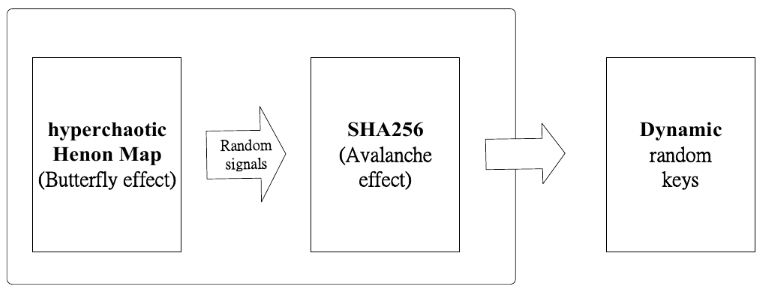
\includegraphics[width=350px]{chapters/res/chapter-2/img/lin.keygen.png}
  \caption{Ilustrasi proses pembangkitan kunci dinamis} \label{fig:lin.keygen}
  Sumber: \textcite{lin2021}
\end{figure}

Proses sinkronisasi sistem \emph{chaos} dapat dilakukan dengan mendekomposisi nilai $u(k)$ menjadi nilai $u_m(k)$ dan $u_s(k)$. Pemecahan nilai ini ditujukan untuk meningkatkan kemananan saat implementasi. Nilai $u_m(k)$ akan dikirimkan dari \emph{transmitter} menuju \emph{receiver}. Sistem ini dapat dijelaskan melalui gambar . Menurut \textcite{lin2021}, sistem itu aman. Hal ini dikarenakan apabla \emph{hacker} memiliki parameter-parameter yang digunakan untuk sinkronisasi, mereka tidak dapat mendapatkan \emph{state} dari master dan slave. Ilustrasi yang proses enkripsi dan dekripsi serta sinkronisasi yang dilakukan terdapat pada gambar \ref{fig:lin.caes}.

\begin{figure}[!h]
  \centering
  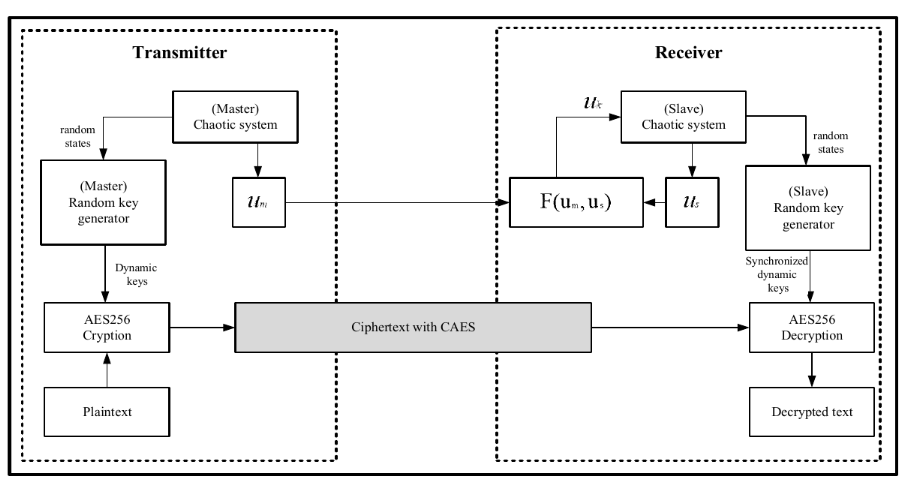
\includegraphics[width=350px]{chapters/res/chapter-2/img/lin.caes.png}
  \caption{Arsitektur AES berbasis \emph{chaos} yang telah diimporvisasi} \label{fig:lin.caes}
  Sumber: \textcite{lin2021}
\end{figure}

Pengujian dari sistem yang dilakukan oleh \textcite{lin2021} adalah dengan cara membandingkan proses enkripsi gambar yang dihasilkan memanfaatkan AES-ECB, AES-CBC, dan CAES-EBC. gambar yang diuji merupakan gambar berukuran $256 \times 256$. Pada algoritme CAES, kunci dinamis yang dihasilkan sebanyak 49.152 kunci. Setiap kunci ini dibuat secara langsung melalui proses \emph{update} pada setiap \emph{round} enkripsi. Hasil enkripsi pada gambar \ref{fig:lin.result} menunjukan bahwa CAES-ECB bila diobservasi secara visual memiliki kualitas yang cukup baik bila dibandingkan dengan AES-EBC. Menurut \textcite{lin2021}, Hal ini dapat membuktikan bahwa algoritme CAES-CBC lebih unggul dibandingkan AES-EBC dan AES-CBC.

\begin{figure}[!h]
  \centering
  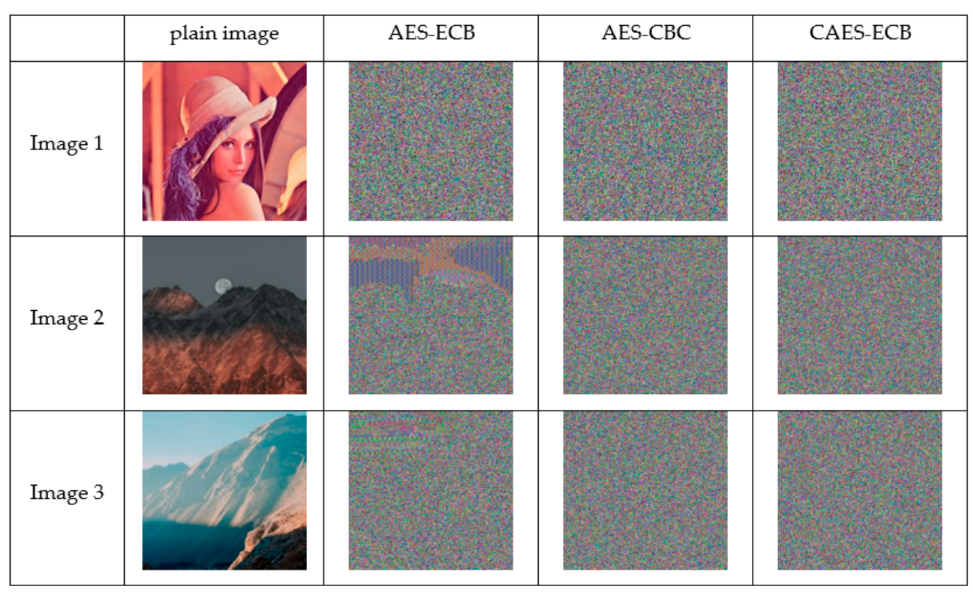
\includegraphics[width=350px]{chapters/res/chapter-2/img/lin.res.png}
  \caption{Hasil visual gambar terenkripsi} \label{fig:lin.result}
  Sumber: \textcite{lin2021}
\end{figure}

Proses enkripsi tersebut juga dilakukan proses pengujian secara analitik. Tes yang dilakukan berdasarkan parameter uji yang telah didefinisikan oleh National Institute of Standards and Technology (NIST). Pengujian yang dilakukan oleh \textcite{lin2021} menggunakan data \emph{stream} sepanjang 10.000.000 bit data dengan jumlah biat setiap stream sebesar 30. Hasil tersebut menunjukan bahwa algoritme CAES memenuhi persyaranan NIST SP 800-22 \emph{random number detection}. Hasil dari pengujian NIST juga menunjukan bahwa algoritme CAES lebih unggul dibandingkan dengan AES-CBC dan AES-EBC. Hal ini ditunjukan dengan data pada gambar \ref{fig:lin.analytic-result}.

\begin{figure}[!h]
  \centering
  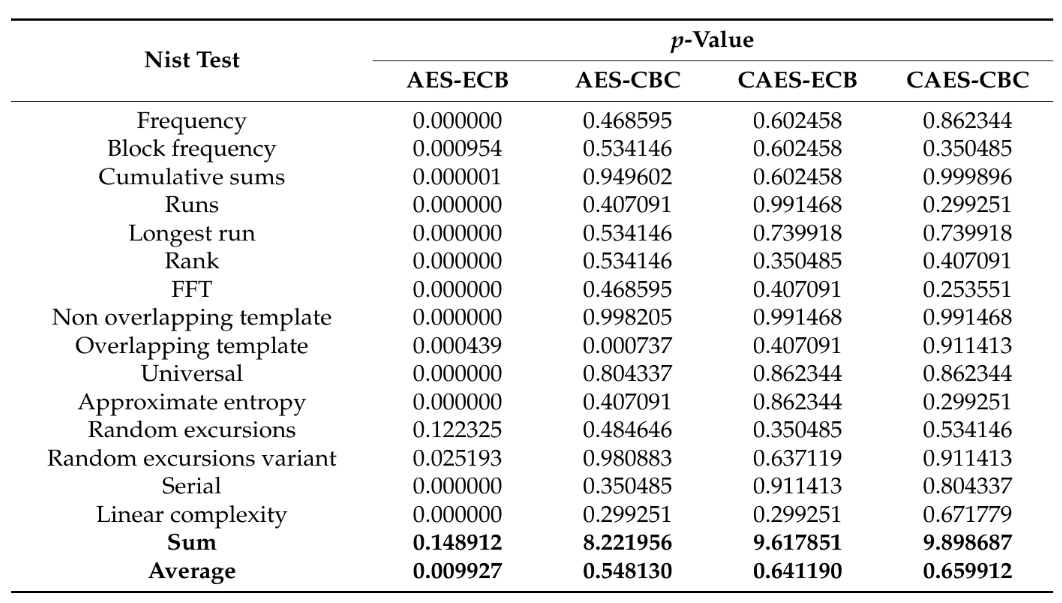
\includegraphics[width=350px]{chapters/res/chapter-2/img/lin.analytic-test.png}
  \caption{Hasil Analitik Algoritme CAES} \label{fig:lin.analytic-result}
  Sumber: \textcite{lin2021}
\end{figure}

\subsection{Enkripsi gambar dan Analisisnya memanfaatkan Algoritme AES dinamis}

Pada penelitian yang dilakukan oleh \textcite{singh2019}, kedinamisan proses enkripsi dilakukan pada S-box. Pada penelitian ini, S-box yang dimiliki oleh AES akan dipermutasi. Terdapat tiga parameter yang digunakan dalam pembentukan S-box ini, yaitu sebagai berikut:
\begin{enumerate}
  \item Kunci\\ Kunci sangat berpengruh terhadap hasil S-box yang dibentuk. Perubahan kecil pada kunci perlu menyebabkan S-box keluaran yang jauh berbeda.
  \item \emph{Irreducible polynomial}\\ Pada penelitian yang dilakukan oleh \textcite{singh2019}, pemilihan \emph{Irreducible polynomial} dilakukan secara acak. Hal ini berbeda dengan algoritme AES pada umumnya yang hanya menggunakan satu polinomial yang digunakan untuk membentuk S-box.
  \item Konstanta Affine\\ Konstanta affine yang digunakan dalam pembentukan S-box. Terdapat 256 konstanta yang dapat digunakan. Dalam penelitian yang dilakukan \textcite{singh2019}, semua konstanta yang dapat digunakan dipilih secara acak untuk membentuk S-box.
\end{enumerate}

Menurut \textcite{singh2019}, S-box yang dapat dibentuk sangat sensitif terhadap tiga parameter diatas. Dengan menggunakan metode tersebut, jumlah kemungkinan S-box dinamis yang dapat dibentuk adalah $256!$. Hal ini dapat memberikan tambahan keamanan pada cipherteks dikarenakan kerumitan tidak hanya berada pada kunci tetapi terdapat pada algoritme.

Pada penelitian \textcite{singh2019}, algoritme enkripsi yang telah dijelaskan sebelumnya diuji dengan melakukan enkripsi gambar \emph{grayscale}. Pengujian yang dilakukan adalah pengujian analisis histogram, pengujian korelasi koefisien, kualitas enkripsi, entropi informasi, dan NPCR-UACI test. Hasil pengujian menunjukan bahwa AES dan Dynamic AES memiliki kualitas enkripsi yang cukup setara. Akan tetapi, dalam pengujian korelasi koefisien, AES dinamis memiliki hasil yang lebih baik dibandingkan dengan AES.

\subsection{Perbaikan Keamanan dari Algoritme AES memanfaatkan \emph{Salt} Dinamis}
Pada penelitian yang dilakukan oleh \textcite{bachtiar2018}, proses enkripsi dinamis dilakukan dengan cara menambahkan \emph{salt} pada pesan yang akan dienkripsi. Nilai \emph{salt} dibuat berdasarkan hasil dari algortima \emph{Linear Congruental Generator} (LCG). Secara global, proses enkripsi dilakukan dengan melakukan proses enkripsi dinamis terlebih dahulu. Setelah itu, proses enkripsi akan dilakukan dengan melakukan AES pada pesan yang telah dilakukan enkripsi dinamis. Proses ini dapat digambarkan pada gambar \ref{fig:bachtiar.enc.process}.

\begin{figure}[!h]
  \centering
  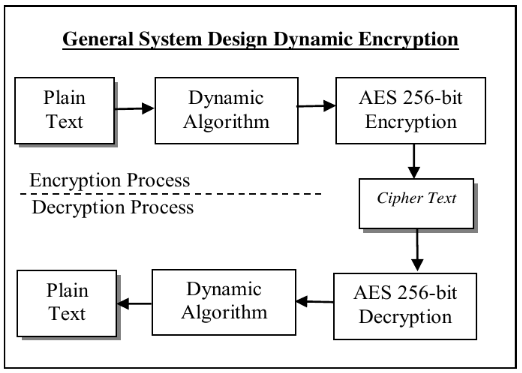
\includegraphics[width=250px]{chapters/res/chapter-2/img/bachtiar.enc.process.png}
  \caption{Ilustrasi proses pembangkitan kunci dinamis} \label{fig:bachtiar.enc.process}
  Sumber: \textcite{bachtiar2018}
\end{figure}

Pada proses enkripsi dinamis, akan dihitung \emph{salt} berdasarkan waktu. Nilai \emph{salt} akan dibuat melalui algoritme LCG.  Nilai salt ini akan ditambahkan pada pesan. Setelah pesan ditambahkan dengan \emph{salt}, pesan akan dilakukan proses enkripsi terlebih dahulu menggunakan OTP. Kunci yang digunakan untuk melakukan OTP merupakan kunci yang sama yang akan digunakan pada proses enkripsi menggunakan AES. Setelah proses ini dilakukan, pesan dinamis tersebut akan dienkripsi menggunakan AES.

Berdasarkan hasil pengujian yang dilakukan menggunakan NIST, teknik memanfaatkan pesan dinamis memberikan hasil yang lebih baik dibandingkan dengan tanpa menggunakan \emph{salt} atapun dengan hanya memanfaatkan \emph{salt} saja. Teknik memanfaatkan pesan dinamis untuk melakukan enkripsi secara dinamis memberikan nilai keberhasilan sebesar $72.5\%$. Nilai keberhasilan ini diperoleh berdasarkan pengujian dengan menjalankan sebanyak delapan kali dan dilakukan perhitungan secara rata-rata.
